\chapter{Results and Discussion}

This chapter presents the major outputs of the study, including the construction of the Akeanon text and speech corpora, and the performance evaluation of the developed ASR model.

\section{Constructed Akeanon Text Corpus}

A total of \textbf{24,000} Akeanon words were collected and verified for the text corpus. This compilation excludes the Swadesh and SIL word lists and includes a wide variety of root words, derivations, and inflections. Figure~\ref{fig:text-corpus} shows a snapshot of the sheet file that serves as the database of the text corpus.

\begin{figure}[H]
    \centering
    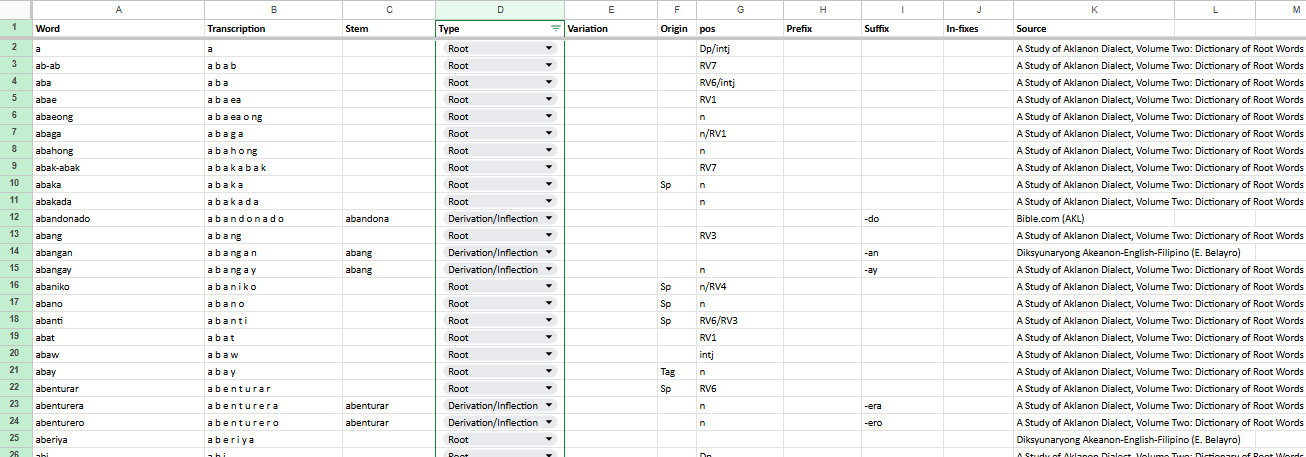
\includegraphics[width=\textwidth]{./figures/text-corpus.png}
    \caption{Snapshot of the Akeanon text corpus}
    \label{fig:text-corpus}
\end{figure}

In addition to the main corpus, the study also translated the Swadesh 207-word list and SIL International's word list into five Akeanon dialects: Standard Akeanon, Bukidnon, Buruangganon, Malaynon, and Nabasnon. Figures~\ref{fig:swadesh-list} and~\ref{fig:sil-list} display sample entries from these translations.

\begin{figure}[H]
    \centering
    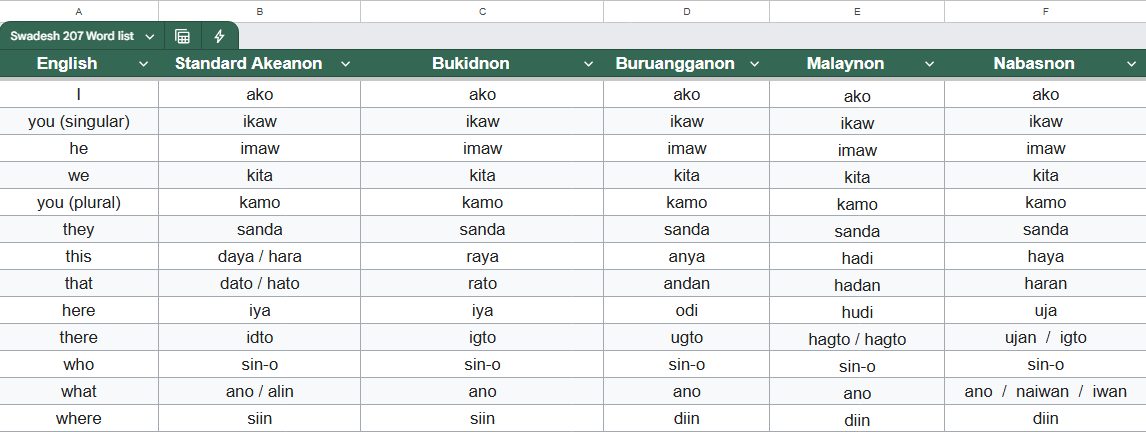
\includegraphics[width=\textwidth]{./figures/swadesh.png}
    \caption{Akeanon translations of the Swadesh 207-word list}
    \label{fig:swadesh-list}
\end{figure}

\begin{figure}[H]
    \centering
    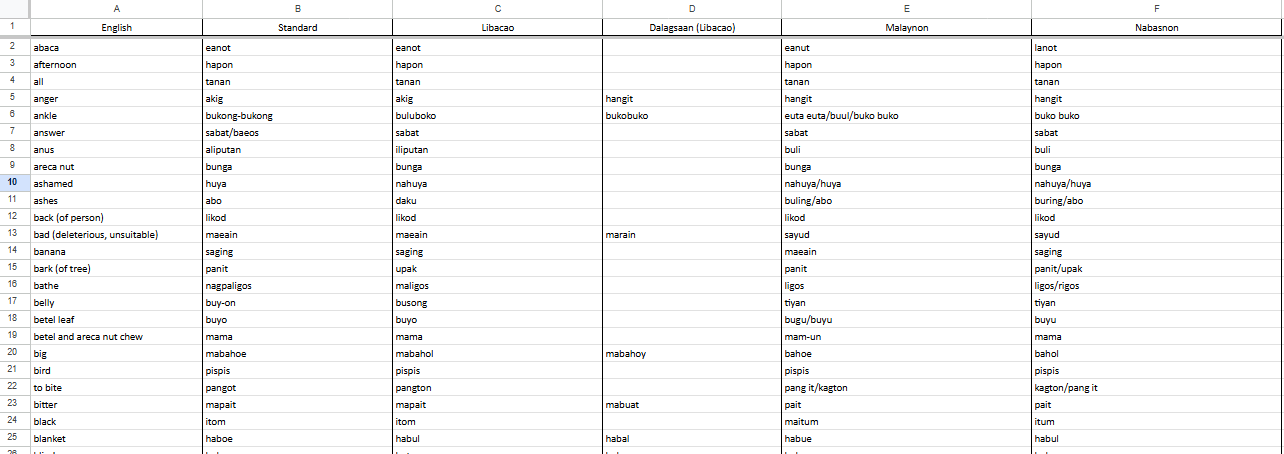
\includegraphics[width=\textwidth]{./figures/SIL.png}
    \caption{Akeanon translations of SIL International's word list}
    \label{fig:sil-list}
\end{figure}

The constructed text corpus serves as a foundation for the development of the Akeanon ASR system, providing linguistic diversity and coverage across different dialects.

\section{Constructed Akeanon Speech Corpus}

For the Akeanon speech corpus, \textbf{100} voice recordings were collected. Each recording corresponds to one of the generated text sets and covers various dialects and speaker demographics.

The collected speech data provides the necessary acoustic material for training, validating, and testing the ASR models. The recordings include natural variations in pronunciation, intonation, and pacing, enriching the acoustic modeling phase.

\section{Monophone and Triphone Model Results}

The monophone and triphone models were trained and evaluated using a ten-fold cross-validation approach.

\subsection{Recognition Performance}

The performance of the models was evaluated based on word recognition accuracy. Table~\ref{tab:accuracy-results} summarizes the results per cross-validation fold.

\begin{table}[H]
    \centering
    \renewcommand{\arraystretch}{1.3}
    \setlength{\tabcolsep}{12pt}
    \caption{Word Recognition Accuracy per Fold}
    \label{tab:accuracy-results}
    \begin{tabular}{|c|c|}
        \hline
        \textbf{Fold} & \textbf{Accuracy (\%)} \\
        \hline
        1 & 85.2 \\
        2 & 86.5 \\
        \hline
    \end{tabular}
\end{table}

\textit{Note: The data above are placeholder values.}
\vspace{1em}

-- to be discussed further --